\section{Illustration}
\label{sec:exps}

To illustrate our theoretical results, we evaluate the predictive performance and the ability of the models to capture the preferential attachment on artificial and real networks. In order to evaluate this property we used several measures.

%We observed the degree distribution and its corresponding best fitting line in log-log scale. In addition, we use the measure developed in \cite{clauset2009power} for assessing whether empirical data behaves according to a power law.

The measures considered to evaluate the preferential attachment rely on a goodness of fit. Indeed, it has been reported that preferential attachment leads to networks characterized by a degree distribution with heavy tail drawn from a power law \cite{barabasi1999emergence}. A graphical method, most often used to verify that the observations are consistent with this law  consists in constructing the histogram representing the degree distribution and if the plot on doubly logarithmic axes approximately falls on a straight line, then one can assume that the distribution follows a power law. Thus, the comparison of the degree distribution in the log-log scale with a linear function gives us a qualitative measure for the preferential attachment. To obtain a second evaluation of the power law hypothesis for the degree distribution, we follow the statistical framework, introduced by \cite{clauset2009power}, for discerning and quantifying power-law behavior in empirical data. This framework combines maximum-likelihood fitting methods with goodness-of-fit tests based on the Kolmogorov-Smirnov statistic. It includes the following steps:


\begin{itemize}
	\item Estimate the parameters $\alpha$ and $x_\text{min}$ of the power law model. $\alpha$ is the scaling parameter of the law and $x_\text{min}$, the lower bound for the tail. It has been fixed to the smallest value observed in the distributions evaluated, in our experiments to allow their comparisons.
	\item  Using the Kolmogorov-Smirnov (KS) statistic, compute the distance $KS_{obs}$  between the degree distribution obtained on the network with the theoretical distribution corresponding to the power law with the estimated parameters.
	\item Sample $S$ synthetic datasets from the power law with the estimated parameters. For each sample  dataset $s \in S$, compute the distance $KS_{s}$ between the distribution obtained on this synthetic dataset, drawn from the power law, with the corresponding theoretical distribution using the Kolmogorov-Smirnov statistic. 
    \item Decide how many sample dataset $S$ to use, with a rule of thumb, based on a worst-case performance analysis of the test \cite{clauset2009power}. To obtain a precision of the $p$-value about $\epsilon$, on should choose $S = \frac{1}{4}\epsilon^{-2}$.  
    \item  The p-value is defined as the fraction of the resulting statistics $KS_s, s \in \{1,...,S\}$ obtained on the samples larger than the value $KS_{obs}$ computed on the network distribution.  
\end{itemize}

 If  p-value is large (close to 1), then the difference between the data and the model can be attributed to statistical fluctuations alone; if it is small, the model is not a plausible fit for the data and we can not conclude that there is an evidence for the preferential attachment in the network. 
However, as mentioned in \cite{clauset2009power} high value of the $p$-value should be considered with caution for at least two reasons. First, there may be other distribution that match the data equally or better. Second, a small number of samples of the data may lead to high p-value and reflect the fact that is hard to rule out a hypothesis in such a case.



%This framework combines maximum-likelihood methods with goodness-of-fit tests based on the Kolmogorov-Smirnov statistics to compute a $p$-value. If the obtained $p$-value is large (close to 1), then the data is likely to be distributed according to a power law and the associated network displays preferential attachment;  on the other hand, if it is small, the data is likely not distributed according to a power law and the associated network does not display preferential attachment.

For local preferential attachment, we follow the same approach as before to compute the $p$-value, the only difference being that the empirical data does not correspond any longer to the global adjacency matrix, but to reduced matrices for each class. The computation of the reduced adjacency matrices varies from one model to the other:

\begin{itemize}
    \item For \imb, for a given class $k$, the reduced adjacency matrix $Y^k$ is defined by:~$y_{ij,k}=1$ if $y_{ij}=1, z_{i\rightarrow j}=z_{i\leftarrow j}=k$ and $0$ otherwise.
    \item For \ifm, the reduced adjacency matrix $Y^k$ is defined by:~$ y_{ij,k}=1$ if $y_{ij}=1 , f_{ik}=f_{jk}=1$ and $0$ otherwise.
\end{itemize}


Note that all our experiments where realized in a platform that we developed and maintain in order to help reproducibility of machine learning experiments. It is available online \footnote{https://github.com/dtrckd/pymake} under a GNU GPL license.

\subsection{Datasets}

To illustrate the above developments, we consider two artificial and two real networks, the characteristics of which are summarized in Table~\ref{table:networks_measures}.


\begin{table}[h] {Characteristics of artificial and real networks.}
    \begin{tabular}{lrrr}
        \hline
        \textbf{Networks} &   nodes &   edges &   density \\
        \hline
        Network1 &    1000 &    3507 &     0.007 \\
        Network2 &    1000 &   31000 &     0.062 \\
        Blogs         &    1490 &   20512 &     0.009 \\
        Manufacturing &     167 &    5950 &     0.215 \\
    \hline
    \end{tabular}
	\label{table:networks_measures}
\end{table}



The non-oriented artificial networks (Network1 and Network2) have been generated with the DANCer-Generator \cite{largeron2015}. This generator has been chosen because it allows one to build an attributed graph having a community structure as well as known properties of real-world networks such as preferential attachment and homophily. In order to test link prediction models on different types of networks, Network1 was generated, by design, to comply with preferential attachment whereas Network2 was not.

The first real network, denoted Blogs \footnote{moreno.ss.uci.edu/data.html\#blogs}, contains front-page hyperlinks between blogs in the context of the 2004 US election. A node represents a blog and an oriented link represents a hyperlink between two blogs. The second one, denoted Manufacturing \footnote{www.ii.pwr.edu.pl/~michalski/index.php?content=datasets\#manufacturing}, is an internal email communication network between employees of a mid-sized manufacturing company. Each node is associated to an employee and an oriented link represents an email sent between the two employees. One can notice that the second network is specific since it is an enterprise network in which the relationships between the employees are (professionally) constrained. This means that this network is less likely to display some of the properties that occur in unconstrained social networks.

The adjacency matrices and global degree distributions of these networks are presented in Figure \ref{fig:corpuses}. This figure allows us to visualize some characteristics of the networks such as their density and their clustering patterns: as one can note, Blogs and the two artificial networks (Network1 and Network2) have a clear community structure, corresponding to the blocks of white dots on the figure, whereas Manufacturing, the denser network, does not have such a structure. Furthermore, the log-log scale plots show that Network1 and Blogs verify the  global preferential attachment (the fitted line represents relatively well the data points) whereas neither Network2 nor Manufacturing verify it. This is confirmed by the $p$-values reported in the first section of Table \ref{table:me_gofit} (Training Datasets): the $p$-value is 1 for Network1 and Blogs, whereas it is null for Network2 and Manufacturing. The parameter $\alpha$ reported in Table~\ref{table:me_gofit} corresponds to the parameter of the estimated power law distribution (\textit{i.e.} the slope of the best fitting line in log-log scale).

Figure \ref{fig:synt_graph_local} represents the local degree distributions for all networks, each curve in each plot being associated to a different class. As the ground truth is not available for the real networks (Blogs and Manufacturing), classes have been determined with Louvain algorithm \cite{Blondel2008} and the local distribution defined according to the obtained classes. As one can note, the plots for Network1 and Blogs are linear for the most frequent degrees, whereas the plots for Network2 and Manufacturing do not display any clear linearity, suggesting that Network1 and Blogs satisfy, at least partly, local preferential attachment whereas Network2 and Manufacturing do not. This is confirmed by the $p$-values reported in Table~\ref{table:me_gofit}: the $p$-value equals  $1$ for Network1 and Blogs,  $0$ for Network2 and $0.4$ for Manufacturing.

\begin{figure}[h]
    \centering
        \begin{minipage}{0.4\textwidth}
            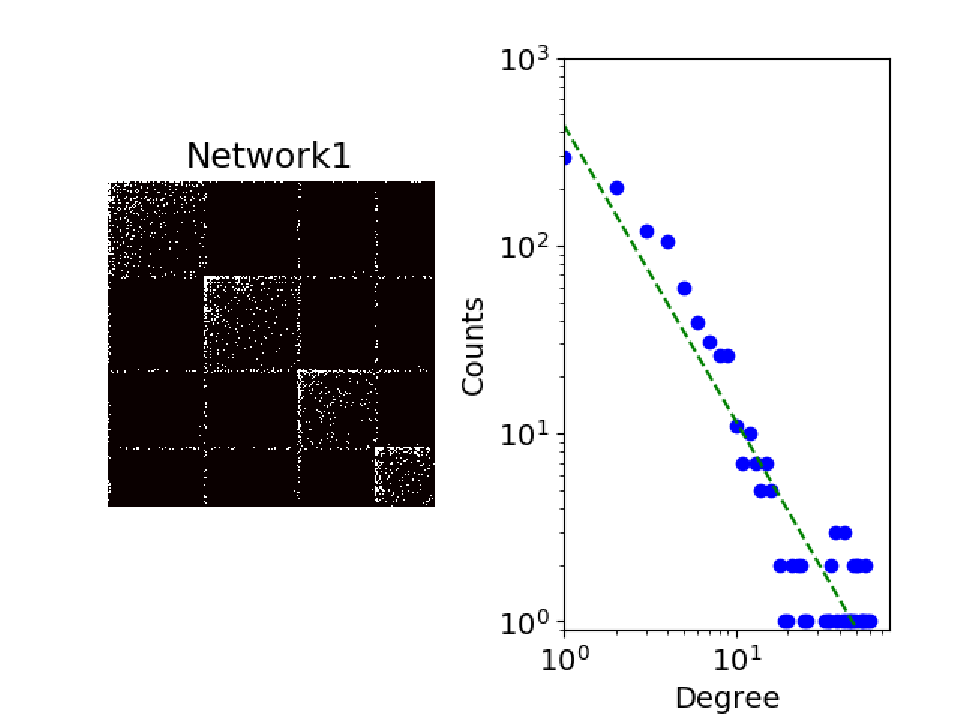
\includegraphics[width=\textwidth]{img/corpus/network1_dd}
        \end{minipage}
        \begin{minipage}{0.4\textwidth}
            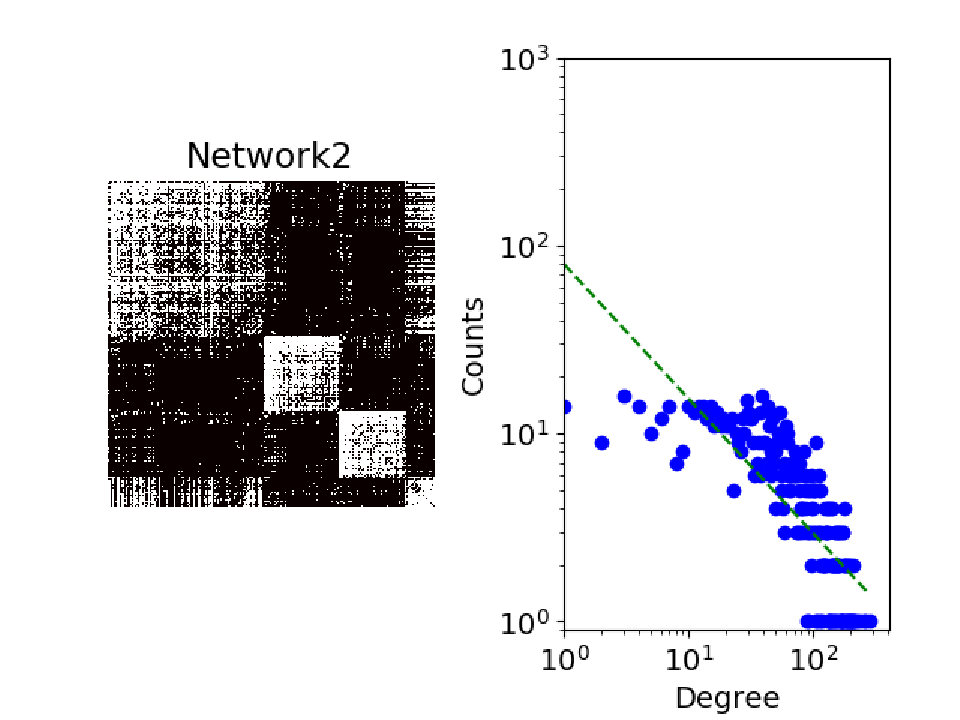
\includegraphics[width=\textwidth]{img/corpus/network2_dd}
        \end{minipage}
        %\vskip\baselineskip
        \begin{minipage}{0.4\textwidth}
            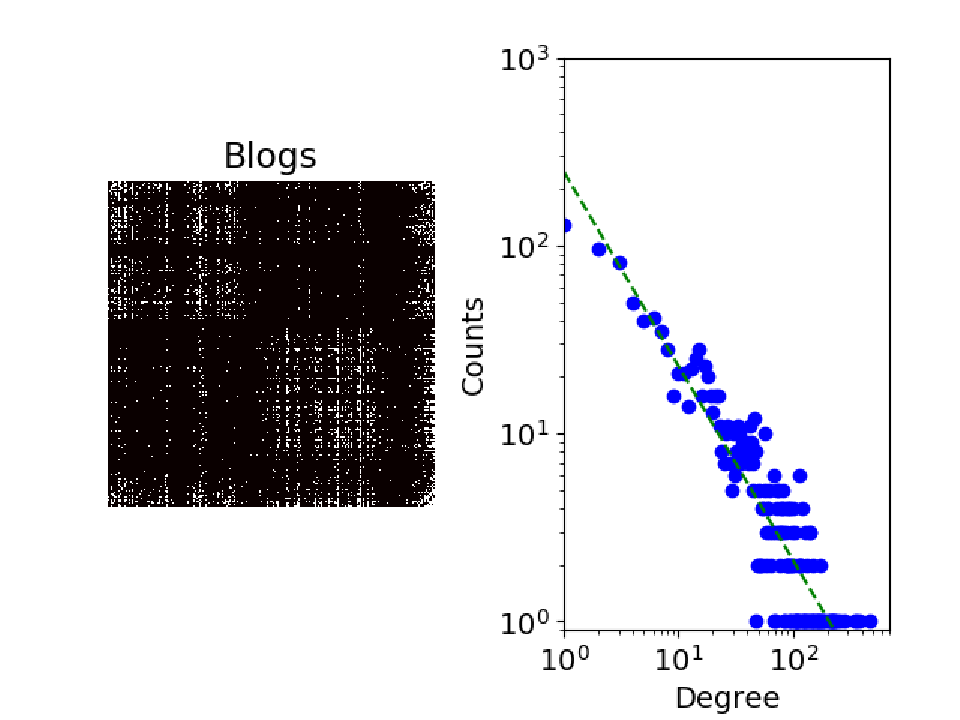
\includegraphics[width=\textwidth]{img/corpus/blogs_dd}
        \end{minipage}
        \begin{minipage}{0.4\textwidth}
            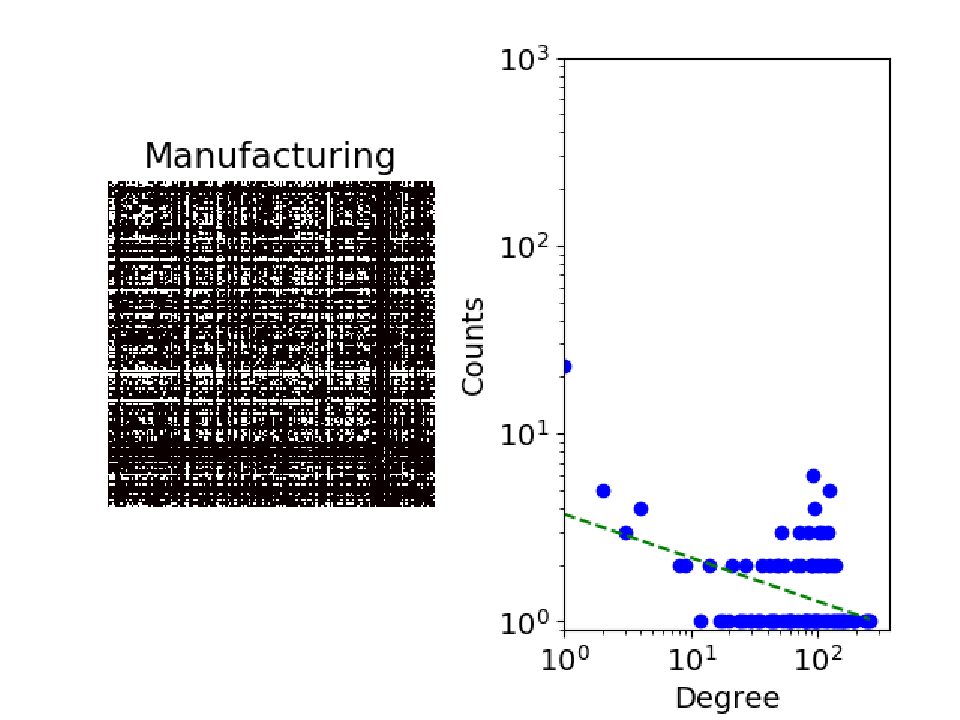
\includegraphics[width=\textwidth]{img/corpus/manufacturing_dd}
        \end{minipage}
	\caption{Adjacency matrices (left) and global degree distributions (right) for the four training datasets. In the adjacency matrices, a white dot corresponds to a 1 and a black dot to a 0.}
	\label{fig:corpuses}
\end{figure}

\begin{figure}[h]
    \centering
        \begin{minipage}{0.4\textwidth}
            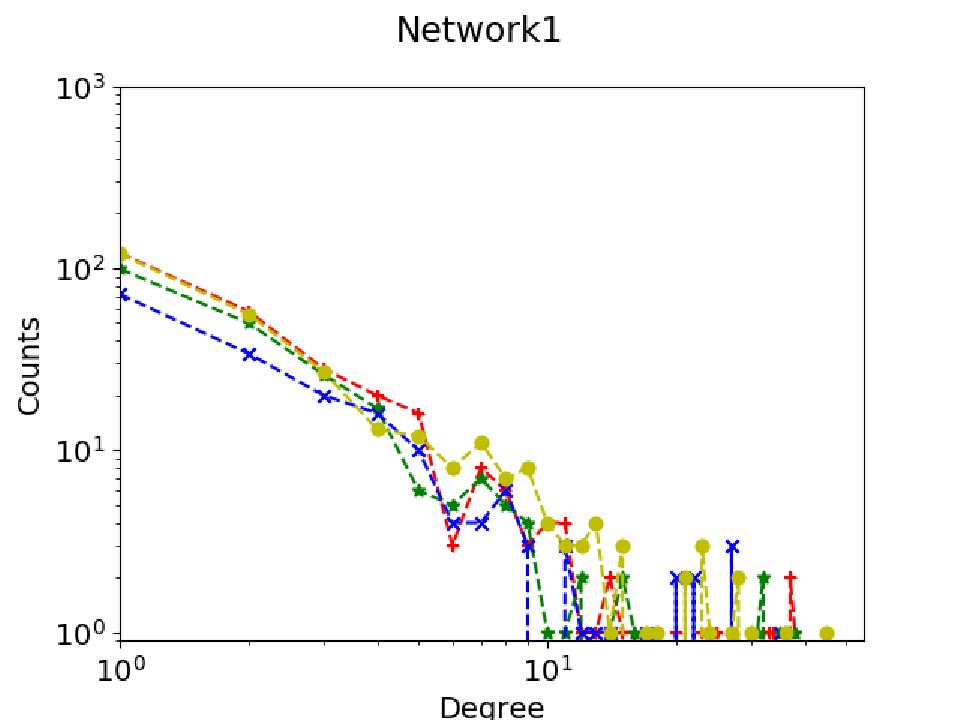
\includegraphics[width=\textwidth]{img/corpus/network1_1}
        \end{minipage}
        \begin{minipage}{0.4\textwidth}
            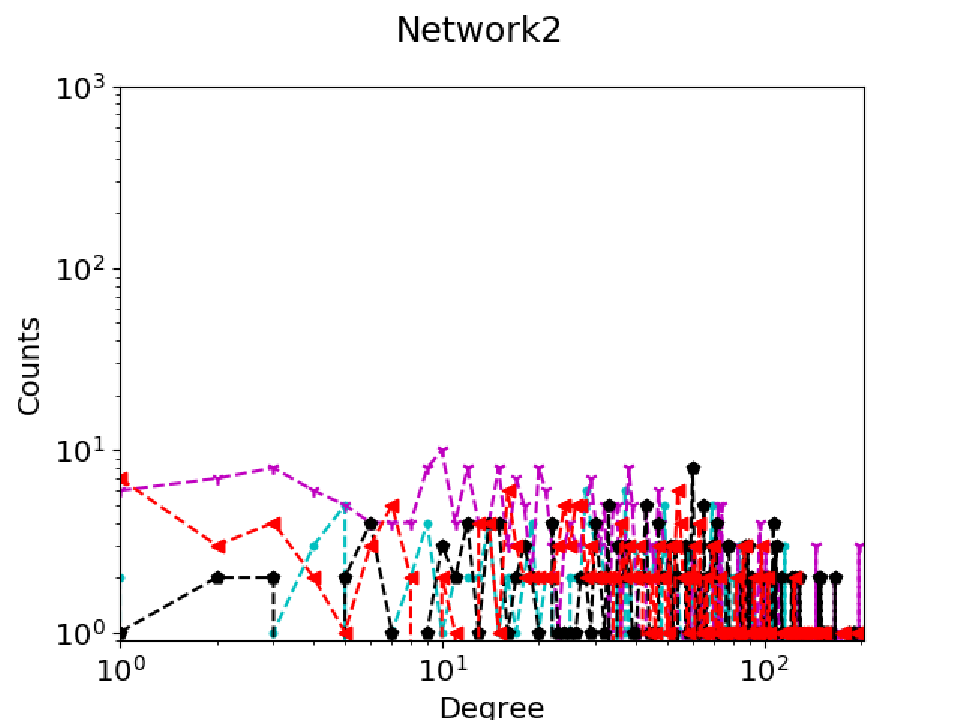
\includegraphics[width=\textwidth]{img/corpus/network2_1}
        \end{minipage}
        \vskip\baselineskip
        \begin{minipage}{0.4\textwidth}
            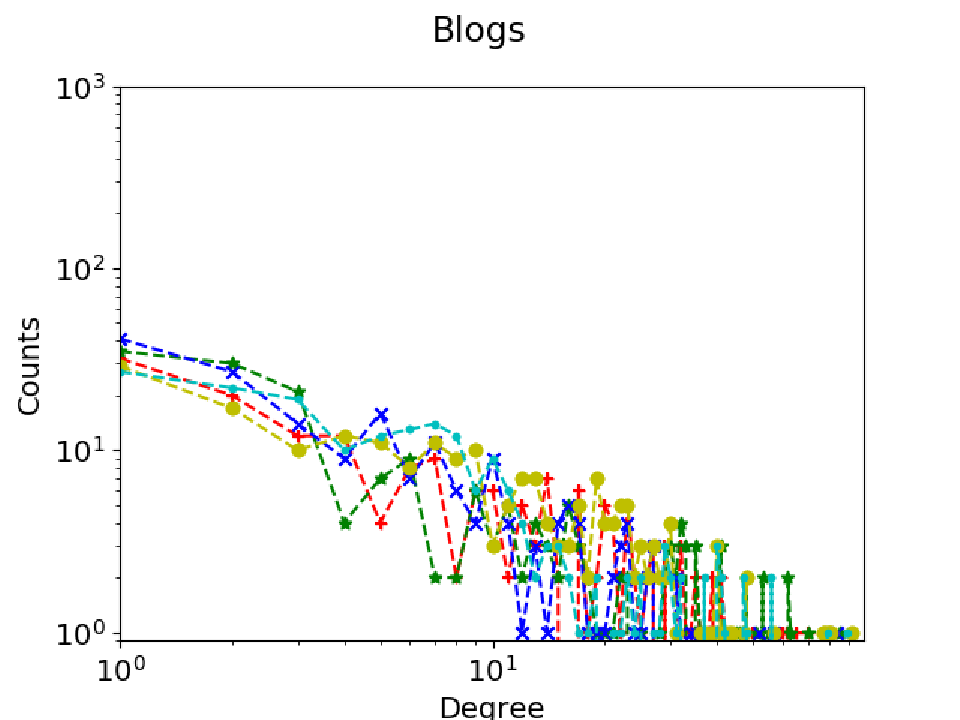
\includegraphics[width=\textwidth]{img/corpus/blogs_1}
        \end{minipage}
        \begin{minipage}{0.4\textwidth}
            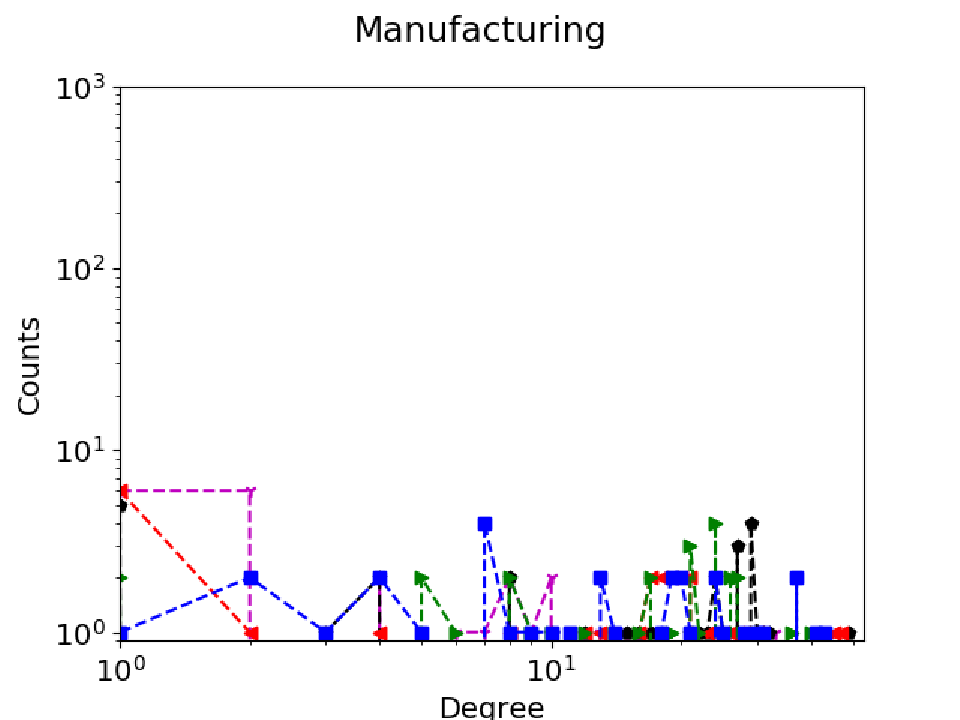
\includegraphics[width=\textwidth]{img/corpus/manufacturing_1}
        \end{minipage}
        \caption {Local degree distributions for the four training datasets. For Network1 and Network2 the classes come from ground-truth. For Blogs and Manufacturing, classes are obtained with a Louvain algorithm.} 
	\label{fig:synt_graph_local}
\end{figure}



\subsection{Preferential attachment in $\M_e$}

For each dataset, we estimated the model parameters through a Markov Chain Monte Carlo inference consisting of 200 iterations. For \imb, the concentration parameters of HDP were optimized using vague gamma priors $\alpha_0 \sim \text{Gamma}(1,1)$ and $\gamma \sim \text{Gamma}(1,1)$ following \cite{HDP}. The parameters for the matrix weights  $\lambda_0$ and $\lambda_1$ were fixed to 0.1. For \ifm, the hyperparameter  $\sigma_w$ was fixed to 1 and the IBP hyperparameter $\alpha$ to 0.5. %in order to  have comparable number of classes with \imb.
Once the models have been learned, they are used to generate links (or non-links) between the entire set of network nodes. The whole procedure is repeated 10 times and the average values are reported as final results.


\begin{table}[h]{Preferential attachment measures for training datasets and networks generated with fitted models.}
\begin{tabular}{lrrrr}
  \multirow{2}{*}{\textbf{Training Datasets}}  &
  \multicolumn{2}{c}{Global} & \multicolumn{2}{c}{Local}\\
  \cmidrule(r){2-3} \cmidrule(l){4-5}
  &   $p$-value &   $\alpha$   & $p$-value & $\alpha$   \\
\hline
Network1       & 1 & 2.4 &   1.0 $\pm$ 0.0  &  1.8 $\pm$ 0.03  \\
Network2       & 0 & 1.3 &   0.0 $\pm$ 0.0  &  1.2 $\pm$ 0.01 \\
Blogs          & 1 & 1.5 &   1.0 $\pm$ 0.0  &  1.4 $\pm$ 0.03\\
Manufacturing  & 0 & 1.4 &   0.4 $\pm$ 0.3  &  1.3 $\pm$ 0.05 \\
\hline

  \ \textbf{\immsb} &&&& \\
\hline
Network1       & 0.9 & 1.4 &   1.0 \(\pm\) 0.0   &  3.5 \(\pm\) 0.7 \\
Network2       & 0 & 1.3 &   0.9 \(\pm\) 0.0   &  1.6 \(\pm\) 0.2 \\
Blogs          & 1 & 1.3 &   1.0 \(\pm\) 0.0   &  4.3 \(\pm\) 1.1 \\
Manufacturing  & 0 & 1.2 &   0.9 \(\pm\) 0.01  &  1.6 \(\pm\) 0.1 \\
\hline

  \ \textbf{\ilfm} &&&& \\
\hline
Network1      & 1 & 1.4 &   1.0 \(\pm\) 0.0  &  1.7 \(\pm\) 0.1 \\
Network2      & 0 & 1.2 &   0.0 \(\pm\) 0.0 &  1.2 \(\pm\) 0.0 \\
Blogs         & 1 & 1.3 &   0.9 \(\pm\) 0.2  &  1.5 \(\pm\) 0.1 \\
Manufacturing & 0 & 1.2 &   0.3 \(\pm\) 0.3  &  1.3 \(\pm\) 0.0 \\
\hline
\end{tabular}
\label{table:me_gofit}
\end{table}


\subsubsection{Degree distributions}

Table \ref{table:me_gofit} reports the value of the power-law goodness of fit for \imb\ and \ifm\ in the global case (left) and in the local case (right). The precision of the test was set to $\epsilon = 0.03$. It appears that for both models, the global preferential attachment is only verified for networks generated from datasets where the property was observed, namely in Network1 with p-value equal to 0.9 for \imb\ and 1 for \ifm, and in Blogs with a p-value equal to 1 for both models; the property is not verified in Network2 and in Manufacturing, where the p-values are equal to 0. This is in accordance with Proposition 2.1 according to which both \ifm\ and \imb\ do not satisfy global preferential attachment. However, these models are able to capture this property if it exists in the training datasets.  Moreover, one can observe that, in the local case, \imb\ complies with the preferential attachment with $p$-values equal or close to 1 for the four networks, while \ifm\ obtained low p-values for the networks that were less locally bursty (respectively  0  for Network2 and 0.3 for Manufacturing). In addition, the power-law coefficients $\alpha$ are significantly greater for \imb\ than for \ifm, and specially for the bursty networks Network1 and Blogs.

Figure \ref{fig:me_local} illustrates the local preferential attachment for Network1 (top) and Network2 (bottom) estimated with \imb\ (left) and \ifm\ (right). The shape of the local degree distributions appears more linear for \imb\ and with more fluctuations for \ifm. This illustrates the fact that \ifm\ does not capture local preferential attachment whereas \imb\ does, as stated in Proposition~\ref{prop:IMBlocal}. 


\begin{figure}[h]
    \centering
    \begin{minipage}{0.4\textwidth}
        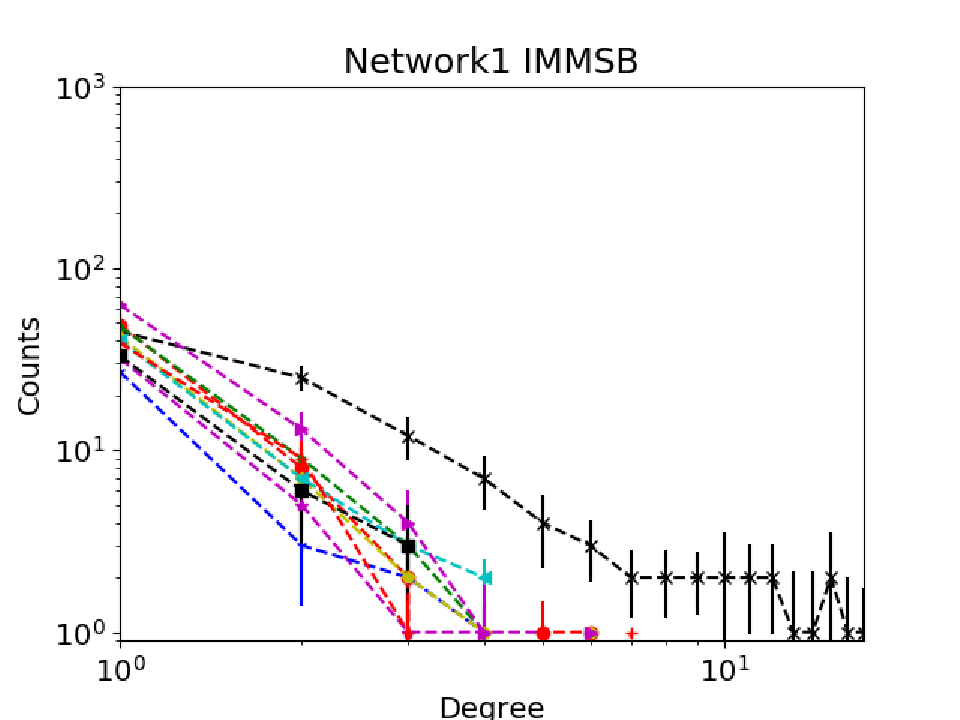
\includegraphics[width=\textwidth]{img/corpus/immsb_network1_1}
    \end{minipage}
    \begin{minipage}{0.4\textwidth}
        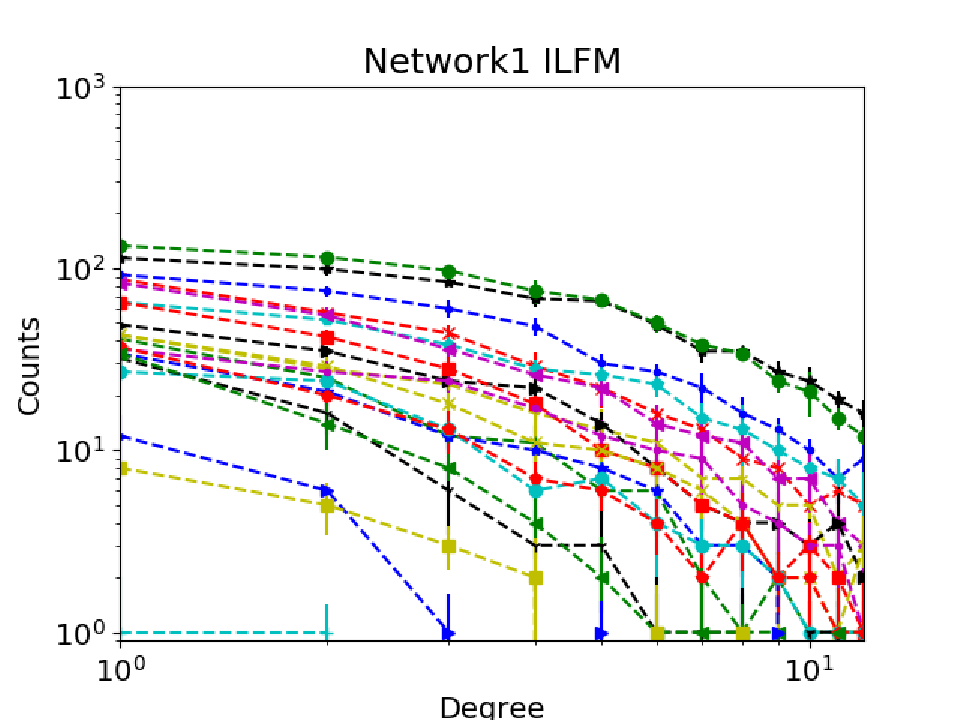
\includegraphics[width=\textwidth]{img/corpus/ilfm_network1_1}
    \end{minipage}
    \vskip\baselineskip
    \begin{minipage}{0.4\textwidth}
        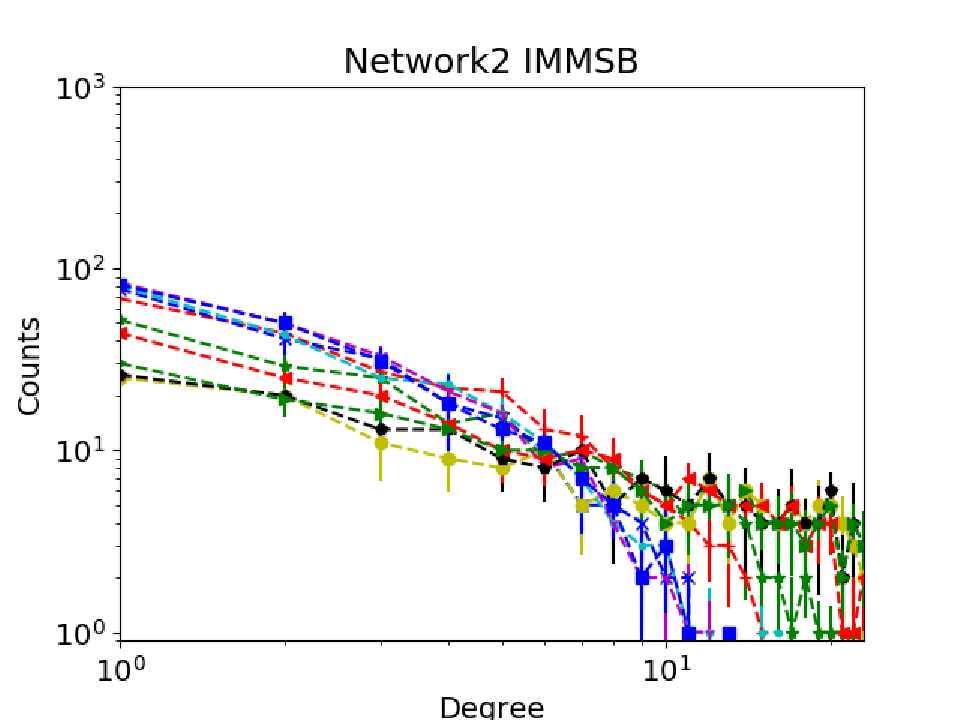
\includegraphics[width=\textwidth]{img/corpus/immsb_network2_1}
    \end{minipage}
    \begin{minipage}{0.4\textwidth}
        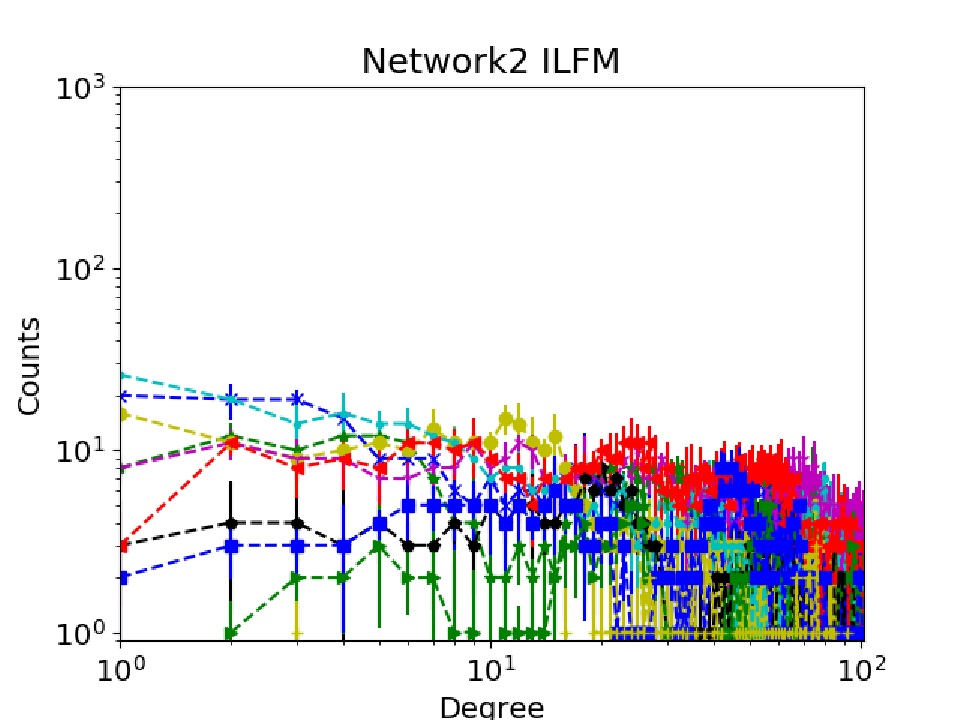
\includegraphics[width=\textwidth]{img/corpus/ilfm_network2_1}
    \end{minipage}
    \caption {Local degree distributions for Network1 (top row) and Network2 (bottom row) generated with fitted models \imb\ (first column) and \ifm\ (second column).} 
\label{fig:me_local}
\end{figure}



\subsubsection{Generating process}
In figure \ref{fig:burst_immsb} and \ref{fig:burst_ilfm} we show respectively for IMMSB and ILFM the evolution of the local preferential attachment following the definition given in section \ref{sec:local_me}, for the networks Manufacturing and Networks1 and for two different values of the generating process step $p$ ($p$ is given as a percentage of $N$ in the plots). For IMMSB one can see on figure \ref{fig:burst_immsb}, that the probability of generating new links increases with the degree. However, for ILFM, one can observe, on figure \ref{fig:burst_ilfm}, some classes where the preferential attachment is no true such as for the class 3 in Manufacturing where the probability to generate new links decreases with the degree or contains some plateau. For Networks1, the probability to generate new links increase in average because the model is fitted with a networks where the preferential attachment is present. However, on can see that the increase of the probability is not as clear than for IMMSB. The value of the probability fluctuate and reach some plateau. The interpretation of these results with regard to the properties that we asses for the local preferential attachment is that IMMSB is better adapted than ILFM to capture the local preferential attachment.


\begin{figure}[h]
\centering

% pmk PNAS3 -x prop2_process_local_me 85 95 -m immsb_cgs -c generator7 manufacturing

\begin{subfigure}
     \centering
         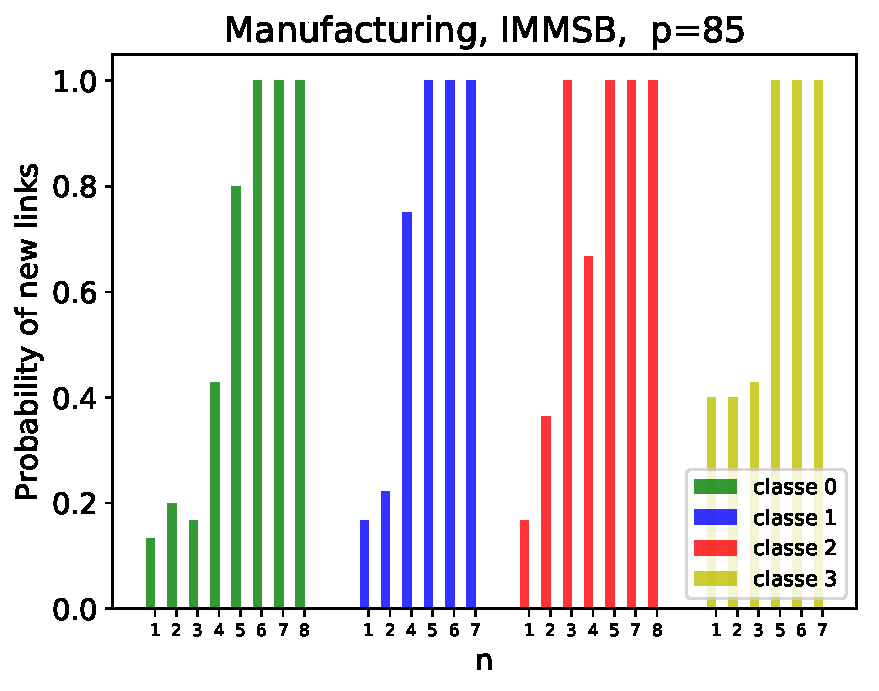
\includegraphics[width=0.45\textwidth]{img/burst/3_prop2_process_local_me__85}
\end{subfigure}
\begin{subfigure}
         \centering
      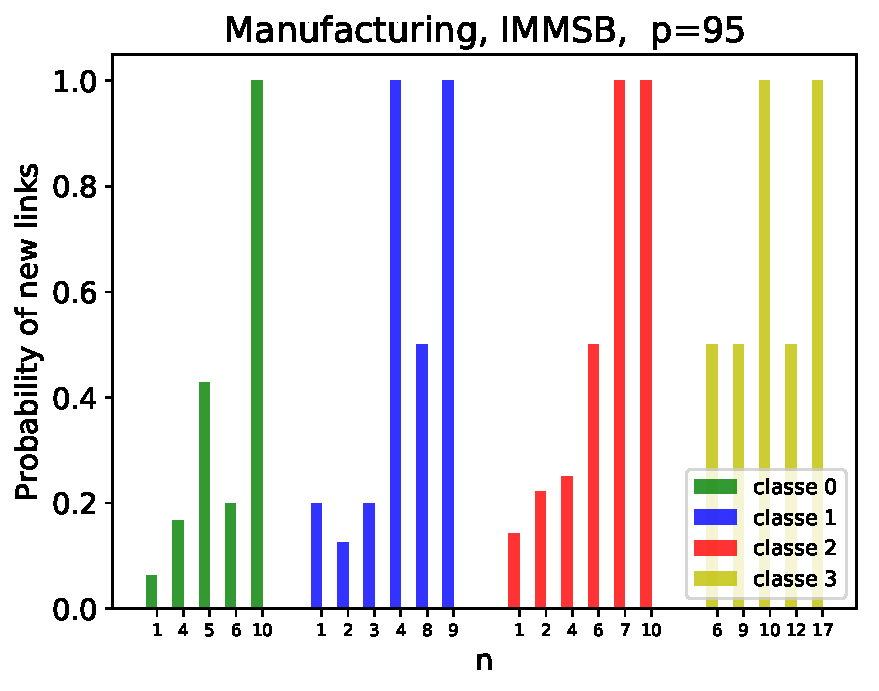
\includegraphics[width=0.45\textwidth]{img/burst/3_prop2_process_local_me__95} 
\end{subfigure}                                                                          
\begin{subfigure}                                                                        
         \centering                                                                      
      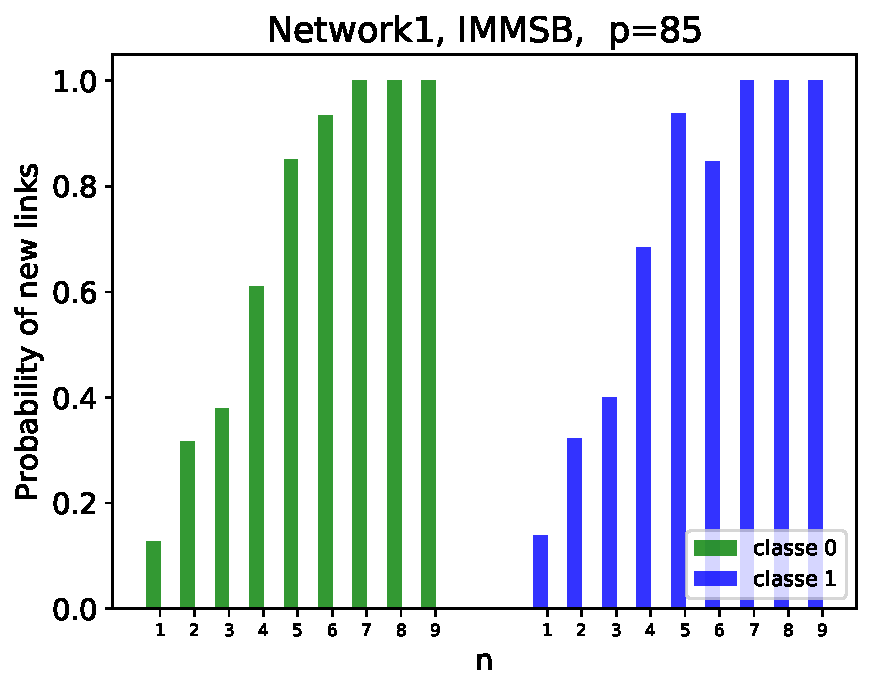
\includegraphics[width=0.45\textwidth]{img/burst/5_prop2_process_local_me__85}
\end{subfigure}                                                                          
\begin{subfigure}                                                                        
         \centering                                                                      
      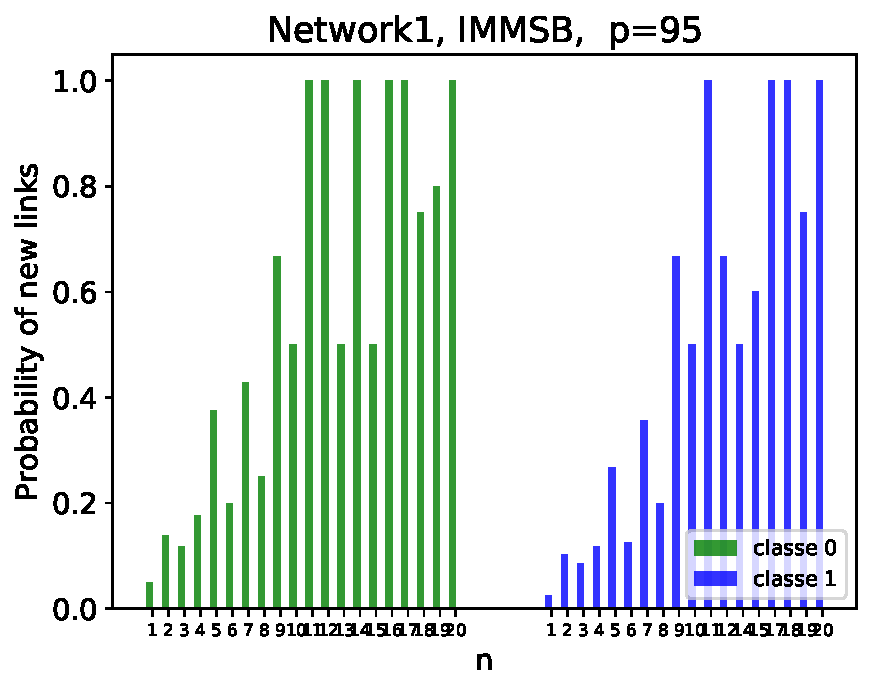
\includegraphics[width=0.45\textwidth]{img/burst/5_prop2_process_local_me__95}
\end{subfigure}                                                                          
\caption{Local burstiness process for IMMSB illustrated by the probability to generate new links for degree at step $p$. The model is fitted with the Manufacturing and networks1 networks for respectively line 1 and 2. First row is for a value of the generating step $p=85\%$(percentage of total number of nodes $N$ and $p=95\%$ for the second row . }
\label{fig:burst_immsb}



\end{figure}

\begin{figure}[h]
\centering

% pmk PNAS3 -x prop2_process_local_me 85 95 -m ilfm_cgs -c generator7 manufacturing 

\begin{subfigure}
     \centering
         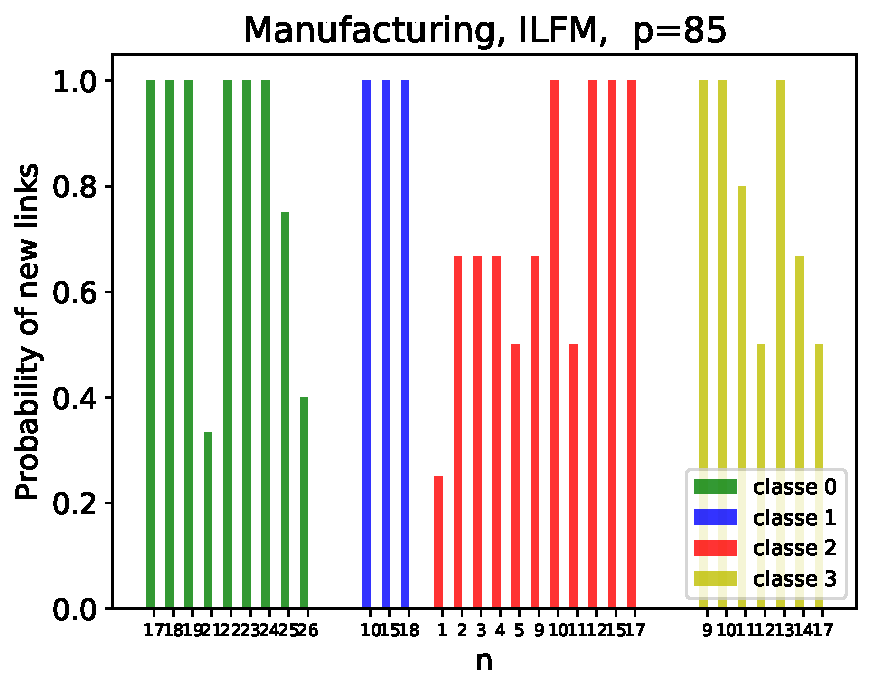
\includegraphics[width=0.45\textwidth]{img/burst/2_prop2_process_local_me__85}
\end{subfigure}
\begin{subfigure}
         \centering
      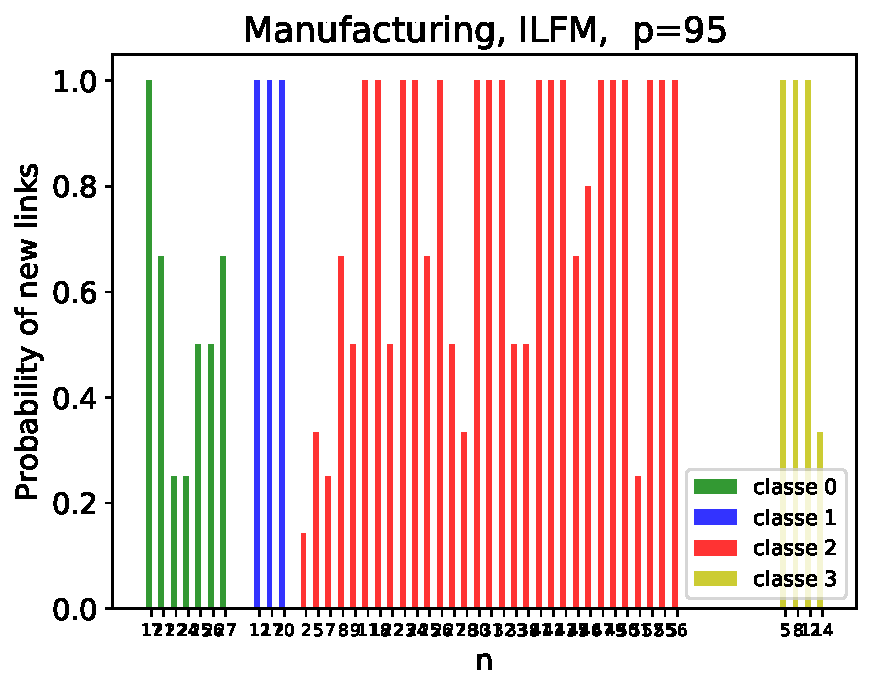
\includegraphics[width=0.45\textwidth]{img/burst/2_prop2_process_local_me__95} 
\end{subfigure}                                                                          
\begin{subfigure}                                                                        
         \centering                                                                      
      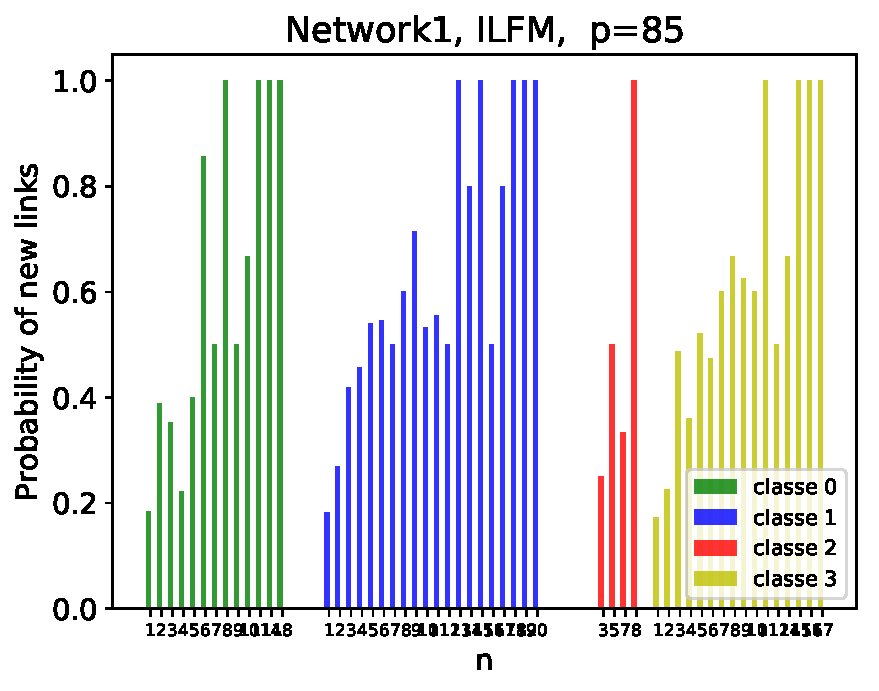
\includegraphics[width=0.45\textwidth]{img/burst/4_prop2_process_local_me__85}
\end{subfigure}                                                                          
\begin{subfigure}                                                                        
         \centering                                                                      
      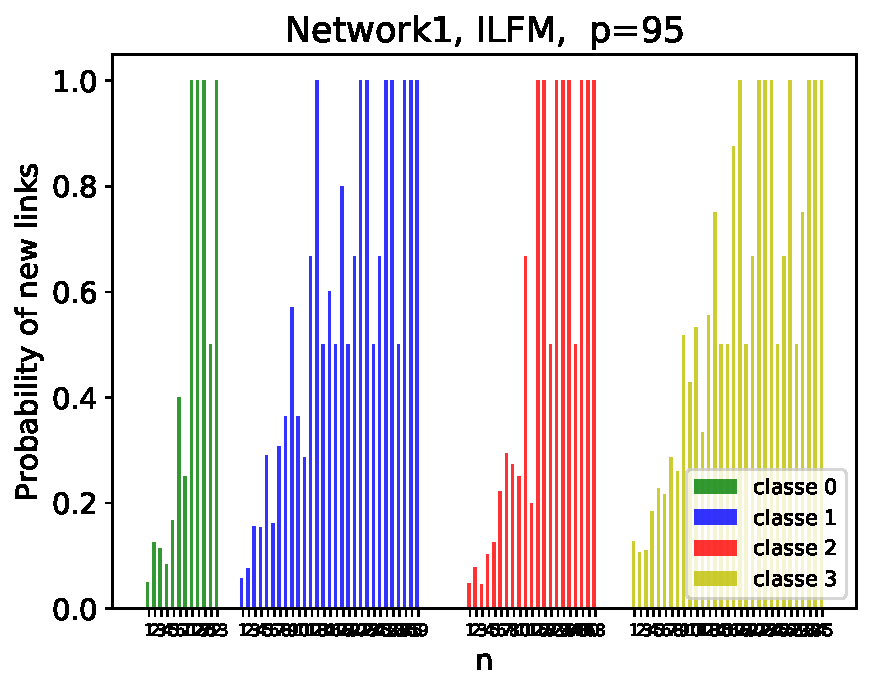
\includegraphics[width=0.45\textwidth]{img/burst/4_prop2_process_local_me__95}
\end{subfigure}                                                                          
\caption{Local burstiness process for ILFM illustrated by the probability to generate new links for degree at step $p$. The model is fitted with the Manufacturing and networks1 networks for respectively line 1 and 2. First row is for a value of the generating step $p=85\%$(percentage of the total number of nodes $N$ and $p=95\%$ for the second row . }
\label{fig:burst_ilfm}



\end{figure}

\subsubsection{Performance evalutation}

%% efficacy != efficiency

Lastly, Figure \ref{fig:auc} compares the performance of the models for predicting new links using the Area Under the Curve (AUC) measure as a function of the training set size. In the bottom plot, the y-axis gives the relative performance defined as the difference of the AUC values for \imb\ and \ifm\ ($AUC_{\imb} - AUC_{\ifm}$) whereas the x-axis indicates the percentage of links randomly removed from the datasets and used as test examples. Hence, the number of training data decreases with the x-axis and a positive value on the y-axis indicates that \imb\ outperforms \ifm.  The relative performance corresponds to the difference of the best AUC values obtained for both models on the 10 inference experiences. The top plots illustrate a case where 75 percent of the data is used as test set and where \imb\ dominates \ifm\ on Network1 (left), and the opposite on Network2 (right).

In general, as shown in the bottom plot, \ifm\ obtains better performance than \imb. However, the relative predictive performance of \imb\  increases  when the quantity of training data decreases on bursty networks, whereas for non-bursty networks the results are the opposite: the performance of \ifm\ increases when the size of the learning dataset decreases. This is particularly visible for Network2. The results for Manufacturing are less marked, which is certainly due to the small size of this network, making the prediction less challenging.

The above behavior can be explained by the fact that \imb\ satisfies the local preferential attachment whereas \ifm\ does not: as links are randomly removed, one is more likely to remove links from large classes than from small ones; a model that enforces local preferential attachment on bursty networks is thus more likely to reconstruct those removed links. This is what is happening on Network1 and Blogs for \imb. On the contrary, for non-bursty networks, a model enforcing local preferential attachment is penalized.

\begin{figure}[ht]
\centering
    \begin{minipage}{0.4\textwidth}
        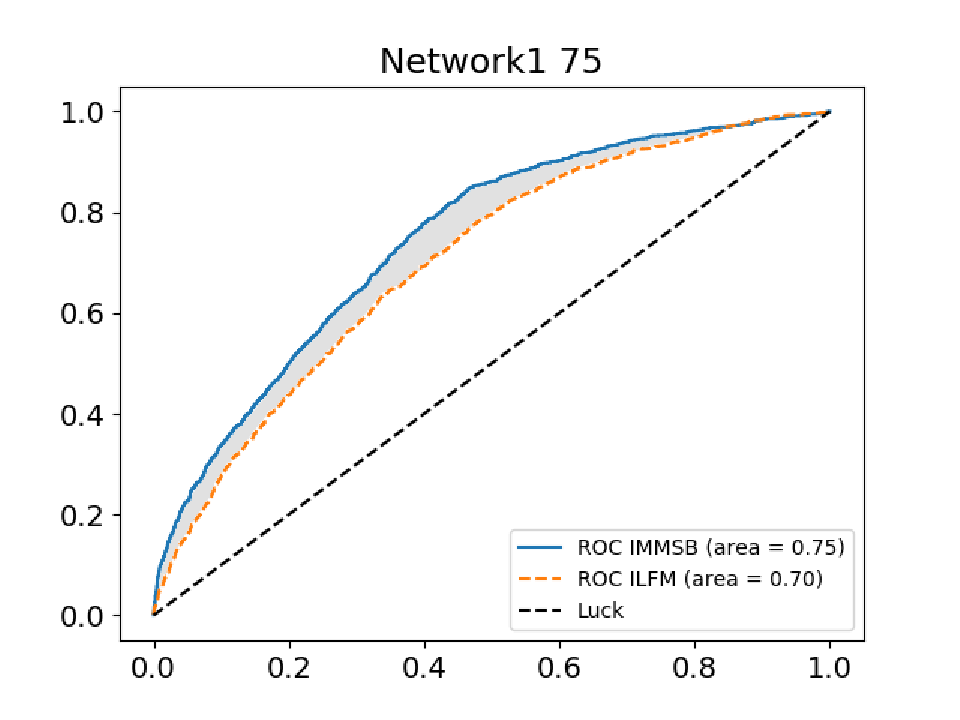
\includegraphics[width=\textwidth]{img/corpus/roc_network1_75_f}
    \end{minipage}
    \begin{minipage}{0.4\textwidth}
        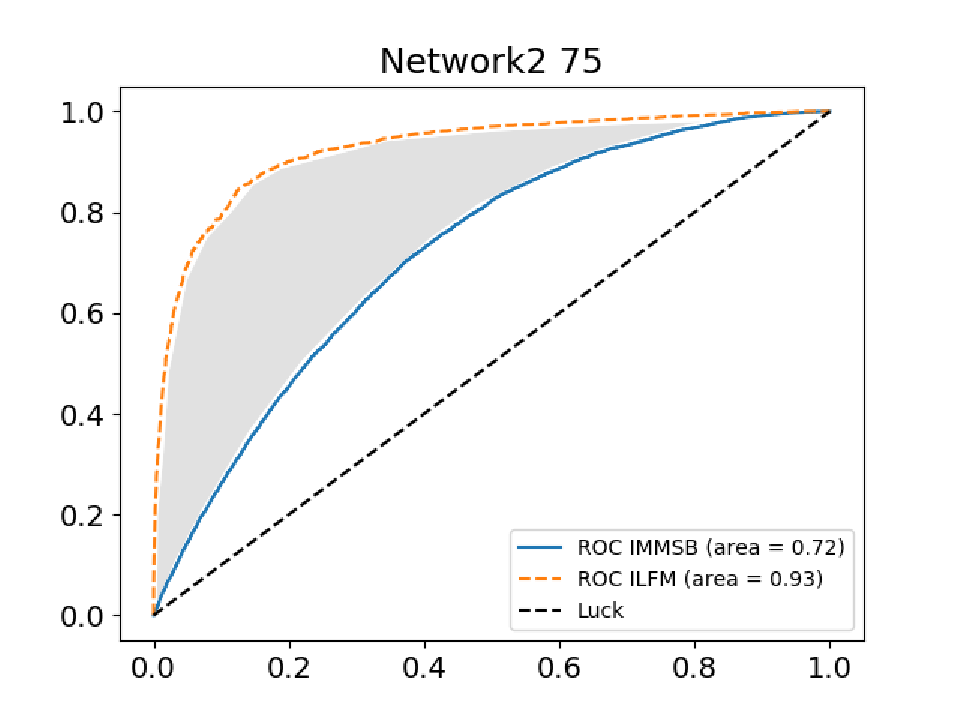
\includegraphics[width=\textwidth]{img/corpus/roc_network2_75_f}
    \end{minipage}
    \begin{minipage}{0.5\textwidth}
        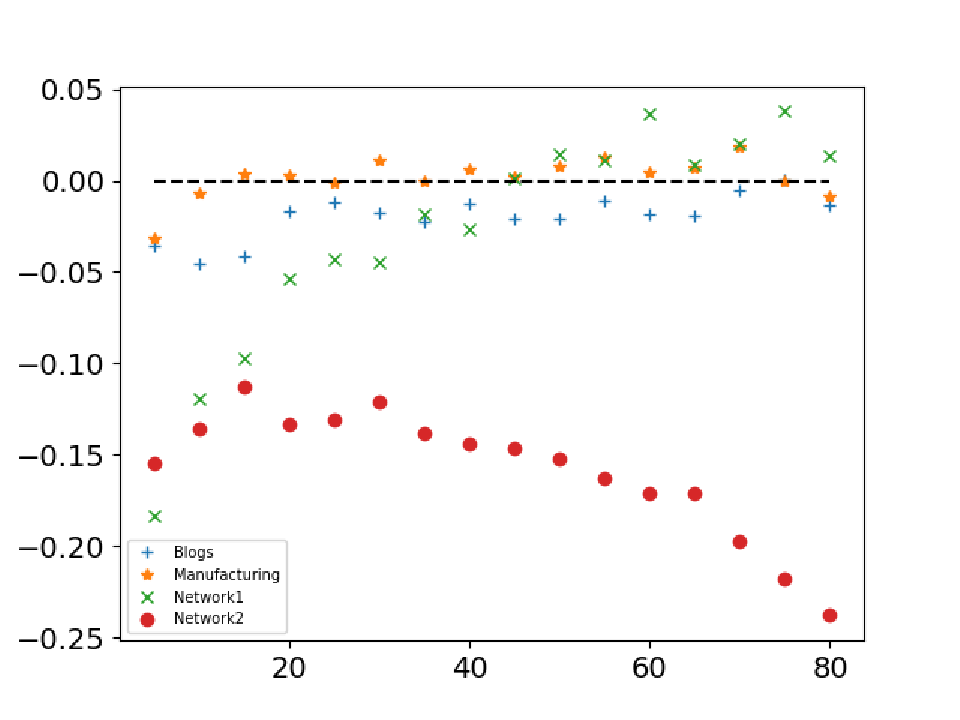
\includegraphics[width=\textwidth]{img/corpus/testset_max_20}
    \end{minipage}
    \caption{Top: AUC-ROC curves for Network1 (left) and Network2 (right) with 75 percent of data used for learning that compares the performance of models. Bottom: Relative performance of \imb\ and \ifm\ according to the percentage of data used for testing, the rest being used for learning.} 
\label{fig:auc}
\end{figure}


\subsection{Preferential attachment in $\M_g$}

Illustrations in the $\M_g$ case are based on the simulation of the models where the parameters $F$ and $\Phi$ have been marginalized out. In other words the degrees that we are going to observe are the expected degree for a large numbers (in the sense of the theory of large numbers) of generated parameters, given the hyper-parameters of the model. In order to simulate this scenario, we generated a large number (100) of networks with a given set of hyper-parameters for the models. Then we reported the average global degree distribution in figure \ref{fig:mg_deg} (top).  For  this  experiments, fix the number of nodes to 1000. We went trough the generative process 100 times in order to simulate the $\M_g$ mode. In order to have a comparable number of classes for \ifm and \imb and block-block probability priors, we fix the hyper-parameters  $\lambda_0=\lambda_1=0.5$ for both models,  $\alpha=\alpha_0=1$ for \ifm, and  $\gamma=0.5$ for \imb.

We see that the global degree distributions are not monotone, with several peaks, and that the range values of the outcome degrees are concentrated in a small segment determined by the hyper-parameters of the models. The shape of the global degree distributions shows that the global preferential attachment is not satisfied. 


In the figure \ref{fig:mg_deg} (bottom), we also reported a measure on the local preferential attachment in $\M_g$. An important note is that, to be able to compute the statistics for the local degree, the latent classes need to be aligned between the different epochs in order to report average values of the local degree distributions. But, the mixed membership models do not defined unique labels over the latent classes. Thus, it is not straightforward to identify the common classes between the generations of the different network realizations. Actually, as the processes are exchangeable, they is no strict correspondence between classes in two independent generative process. Nevertheless, the property of the Dirichlet Process and the Indian Buffet Process, enable to identify the classes by ordering them with their size (or concentration). For example, the stick breaking process interpretation of the DP provides a natural class ordering with a descending (or ascending) order of the class representations. While the IBP generates a row-exchangeable feature matrix, it is possible to reorder the rows to obtain a $F$ matrix where the size of the classes keeps the same descending (or ascending) order.

For the local degree, one can see that, for IMMSB, the shape of the distributions is characteristic of the preferential attachment effect (linear decrease in a log-log space) while it is not the case for ILFM. This experiment is interesting as it show that, for \imb, the local preferential attachment property in $\M_e$ seems to holds also in $\M_g$.

% Degree distribution in MG
%  2x2 figure  
%  [global immsb] [global ilfm]
%  [local ilfm] [gloal ilfm]
%
% pmk PNAS3 -x gennetwork burstiness -g -c generator7 -n 1000 --epoch 100


\begin{figure}[h]
    \centering
    \begin{minipage}{0.45\textwidth}
        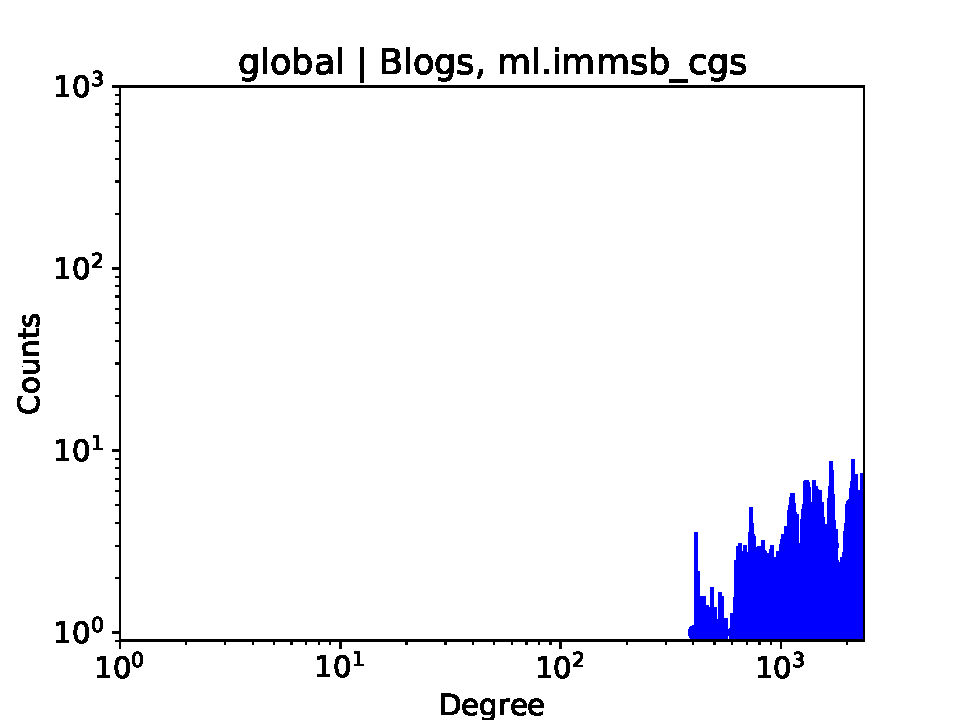
\includegraphics[width=\textwidth]{{{img/0201/MG_ml.immsb_cgs_0}}}
    \end{minipage}
    \begin{minipage}{0.45\textwidth}
        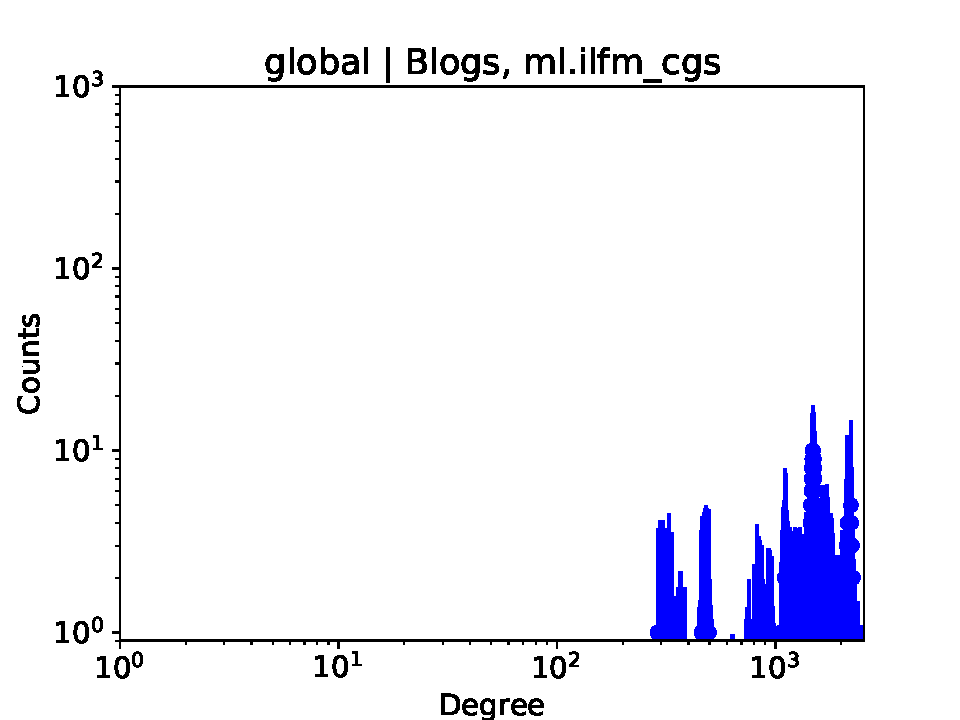
\includegraphics[width=\textwidth]{{{img/0201/MG_ml.ilfm_cgs_0}}}
    \end{minipage}
    \vskip\baselineskip
    \begin{minipage}{0.45\textwidth}
        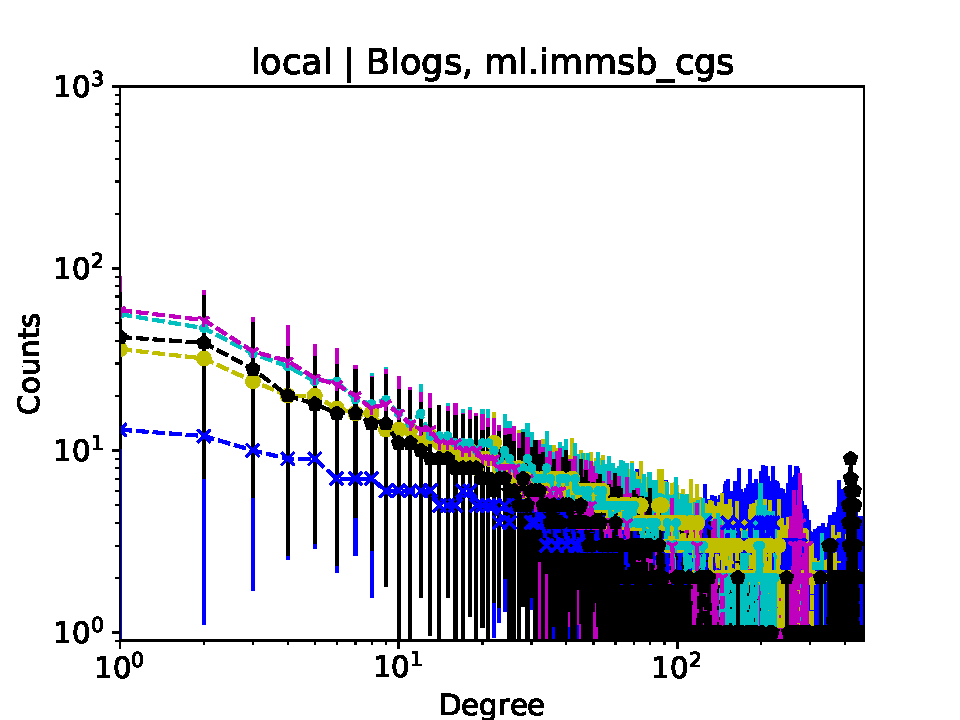
\includegraphics[width=\textwidth]{{{img/0201/MG_ml.immsb_cgs_1}}}
    \end{minipage}
    \begin{minipage}{0.45\textwidth}
        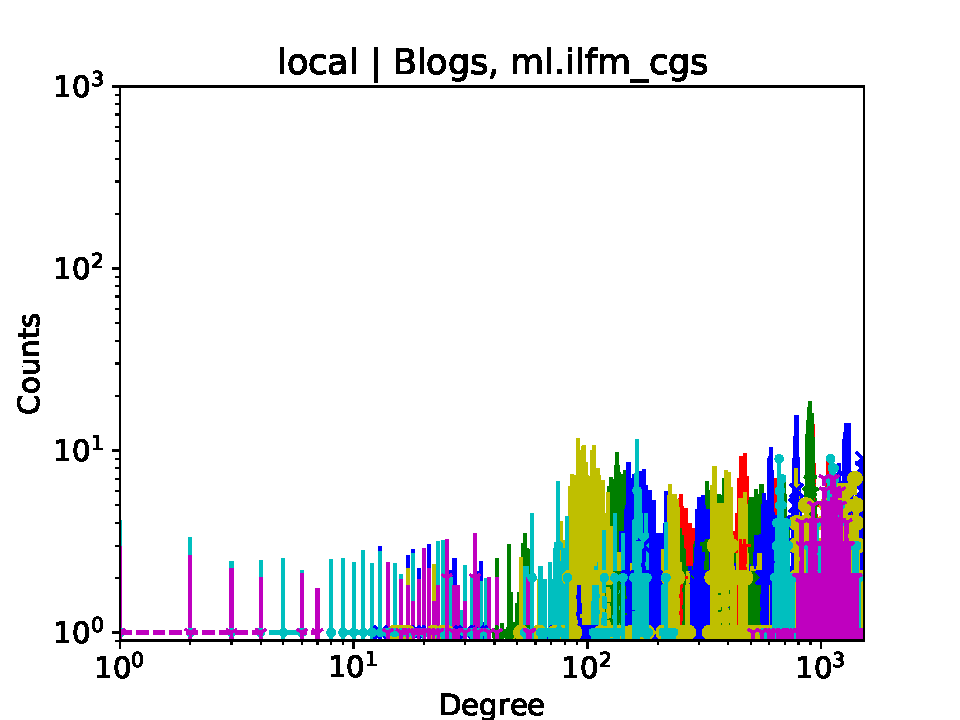
\includegraphics[width=\textwidth]{{{img/0201/MG_ml.ilfm_cgs_1}}}
    \end{minipage}
    \caption {Global degree distribution (top) and local degree distribution (bottom) from IMMSB (left) and ILFM (right) in the generative mode $\M_g$.} 
\label{fig:mg_deg}
\end{figure}



%Figures \ref{fig:mg_process} gives a simulation of the evolution of the expected (global and local) degree during the sampling process according to the equation \eqref{eq:degree_def}. We will refer this process as the degree count process which basically is a cummulative count over the nodes of the link measure (eitheir the true link/non-link observation for ILFM or the likelihood of a link for IMMSB) . Because, we observe the degree count averaged on all the nodes, we also plot the variance over the nodes of those degree count process.
%Interestingly, one can show that for both models, the global and local expected degree count processes follow a linear increase, while the variance of the degree count processes are slightly convex. Furthermore, it is more pronounced for IMMSB for the global degree while it seems that concerning the local degree, the models are not differentiable. Nevertheless, if we look at the standard deviation of the variance for each local degree we see that for IMMSB it seems to be correlated to the variance (the more variance (over nodes) in a local degree count, the more this variance can deviate. In other words, the variance over the epoch increase too.). This is an interesting interpretation of the source of emergence of the local preferential attachment for IMMSB.

%% Degree process (cumulative count) in MG
%  2x2 figure  
%  [glogal expectaion] [global variance]
%  [local expectation] [local variance]
%
% pmk PNAS3 -x burst_process_mg -g -c BA -n 200 --epoch 10
% pmk PNAS3 -x burst_process_local_mg -g -c BA -n 200 --epoch 100


\begin{figure}[h]
    \centering
    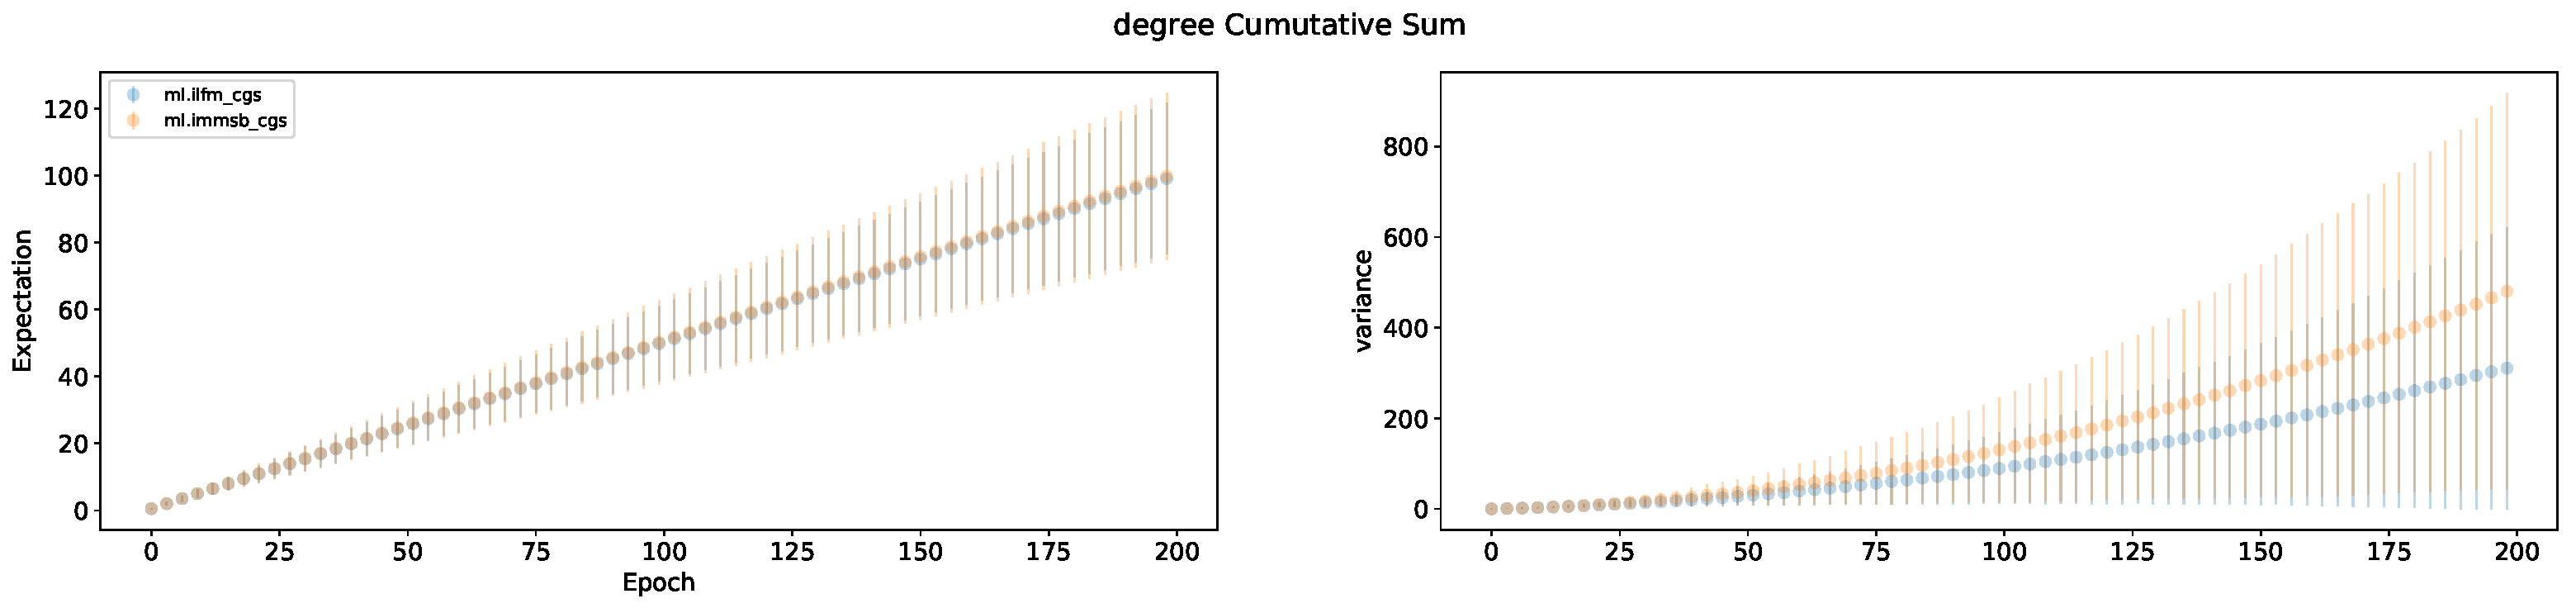
\includegraphics[width=\textwidth, height=6cm]{{{img/0201/BA_burst_process_mg_BA}}}
    \caption {The Left plot is the expectation of the degree count process over the nodes of the network. The right plot is the variance of the degree count process over the nodes of the network. The standard deviation of the curves is the deviation according to each epoch generation.} 
\end{figure}

\begin{figure}[h]
    \centering
    \begin{minipage}{0.99\textwidth}
        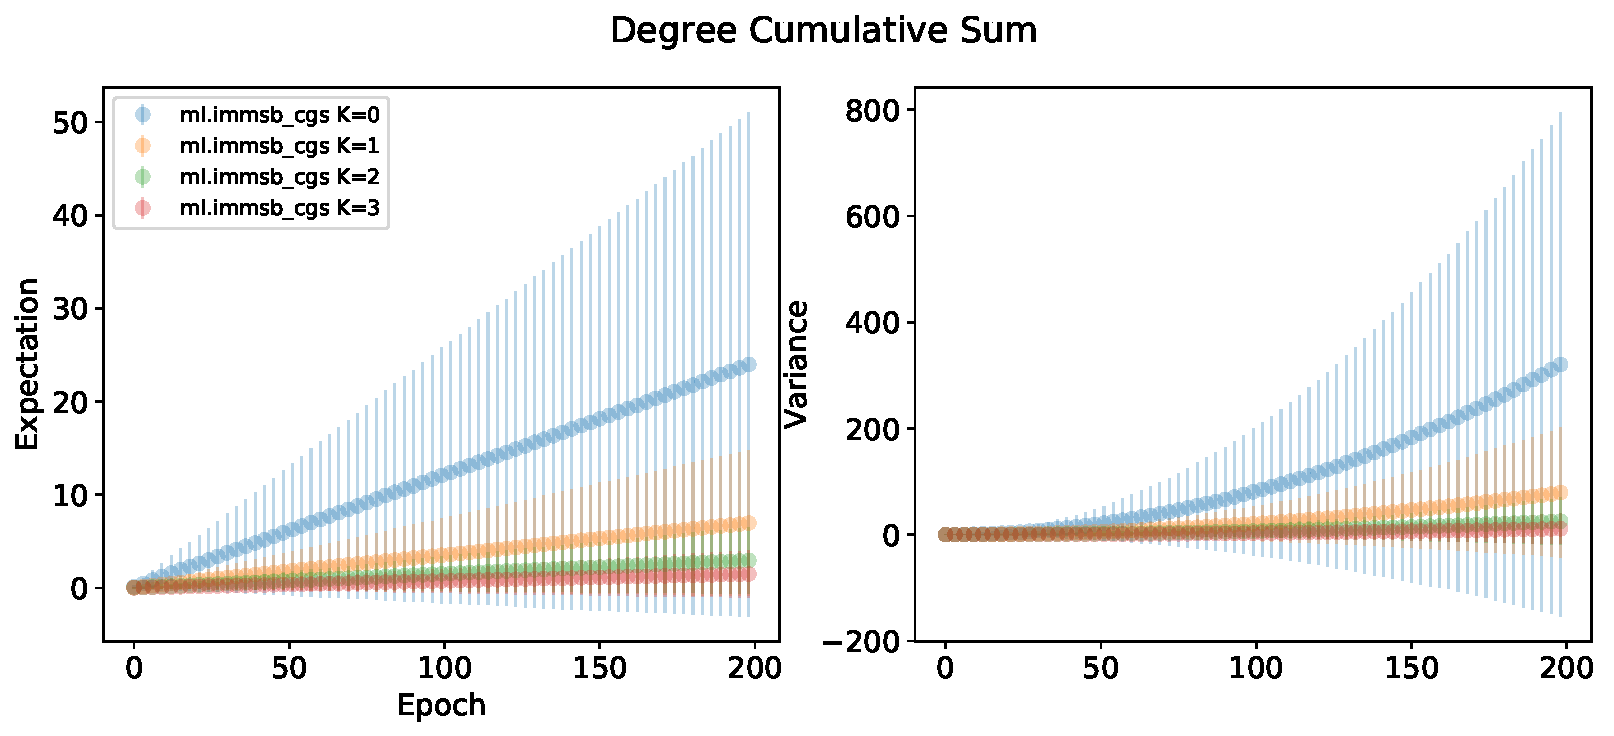
\includegraphics[width=\textwidth]{{{img/0201/ml.immsb_cgs_burst_process_local_mg_ml.immsb_cgs}}}
    \end{minipage}

    \begin{minipage}{0.99\textwidth}
        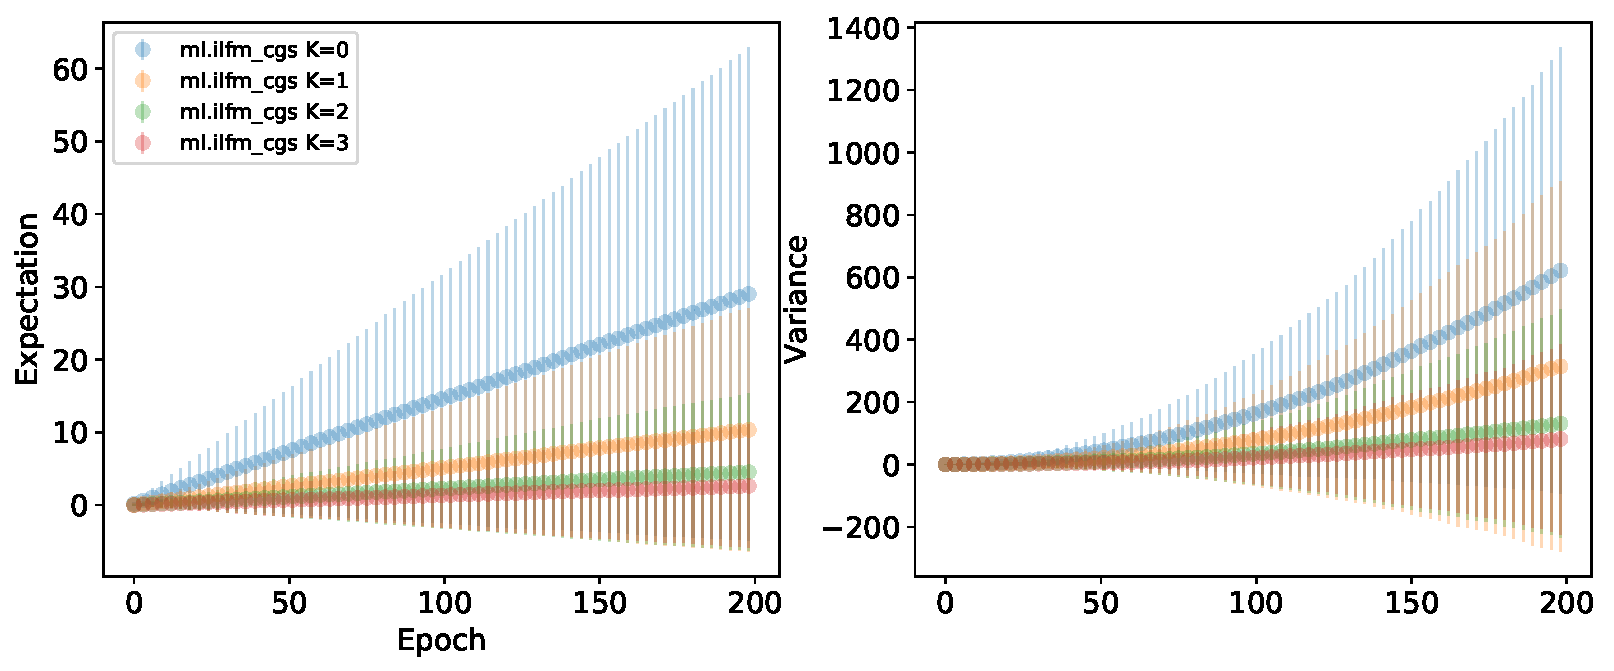
\includegraphics[width=\textwidth]{{{img/0201/ml.ilfm_cgs_burst_process_local_mg_ml.ilfm_cgs}}}
    \end{minipage}
    \caption {Top figure represent IMMSB local degree count process. The left part of the figure is the average overs the network's node and the roght part is the variance. Bottom figure is the same quantities but for ILFM model.} 
\label{fig:mg_deg}
\end{figure}




